%
% Documento: Metodologia
%
\chapter{Metodologia}
\label{chap:Metod}
Para a realização deste trabalho, primeiramente fez-se um estudo das estratégias de controle de formação de robôs móveis, das possibilidades de implementação dessas estratégias na plataforma a ser utilizada (no caso, o \emph{Lego Mindstorms\textregistered}) e da viabilidade de modelar e implementar o sistema como um sistema distribuído descentralizado. Neste tipo de topologia de comunicação não há um mestre definido, apenas uma sociedade de robôs que conforme precisam executar uma tarefa, vão se coordenando e formando um sistema multiagente. 

Após realizados os estudos, concluiu-se que, apesar de viável como pode ser visto no capítulo \ref{chap:trabalhosRelacionados}, a implementação de um sistema distribuído descentralizado seria muito complexa para ser abordado no período proposto para a realização deste trabalho, que tem como objetivo principal o estudo de estratégias de controle de formação de múltiplos robôs móveis. Para tanto, foi adotada uma estrutura de rede centralizada do tipo 'Mestre/Escravo', utilizando o protocolo de comunicação \emph{bluetooth}, o qual é suportado pela plataforma e pela linguagem \emph{NXC}.%a comunicação via \emph{Bluetooth}, a qual a própria plataforma e linguagem (\emph{NXC}) dão suporte. 

%Além disso, será feito um controle em cascata, onde a saída de um módulo de controle  utilizado para modularizar o problema e assim, tornar mais simples a implementação e o entendimento do mesmo. %Ponto?
%Além de facilitar na validação do sistema, que foi implementado da malha mais interna à malha mais externa, sendo testado e validado módulo à módulo de controle, bem como suas integrações.  %Para facilitar a implementação, a modelagem foi implementada em módulos de controle, com o intuito de simplificar o entendimento e a validação do sistema. A implementação foi feita da malha mais interna à malha mais externa, sendo testado e validado módulo à modulo de controle, bem como suas integrações.

Existem diversas maneiras de se implementar um sistema como este, tanto do ponto de vista do sistema distribuído e sua rede de comunicação, quanto do ponto de vista de controle e realimentação das malhas. Foram escolhidos dois tipos de formações diferentes e uma estratégia que pode ser adaptada para ambos os problemas. %Foram escolhidas duas estratégias diferentes de formação de múltiplos robôs móveis %e fez-se então, duas abordagens distintas. Uma delas que atende apenas à um dos problemas e uma outra abordagem mais genérica que pode ser adaptada para a resolução de ambos os problemas. 

Para estabelecer o modelo matemático do problema, foi considerado o modelo de robô mostrado na \autoref{fig:robo}, que consiste em um modelo não holonômico, onde tem-se duas rodas unidirecionais e uma roda orientável. Para definição do modelo matemático levou-se em consideração que os \emph{encoders} seriam utilizados para odometria e então, foram definidas as restrições da modelagem matemática do problema que, desconsidera problemas como: saturação do atuador, derrapagem das rodas, os erros de medição dos \emph{encoders}, bem como as limitações da plataforma. %Tendo em vista um levantamento das dificuldades que surgiram somente na implementação do sistema no mundo real, foi-se adaptando as soluções para o problema e o problema, de forma a viabilizar a correção de erros de sensoriamento que se acumulam a cada iteração.

\begin{figure}[!htb]
	\centering
	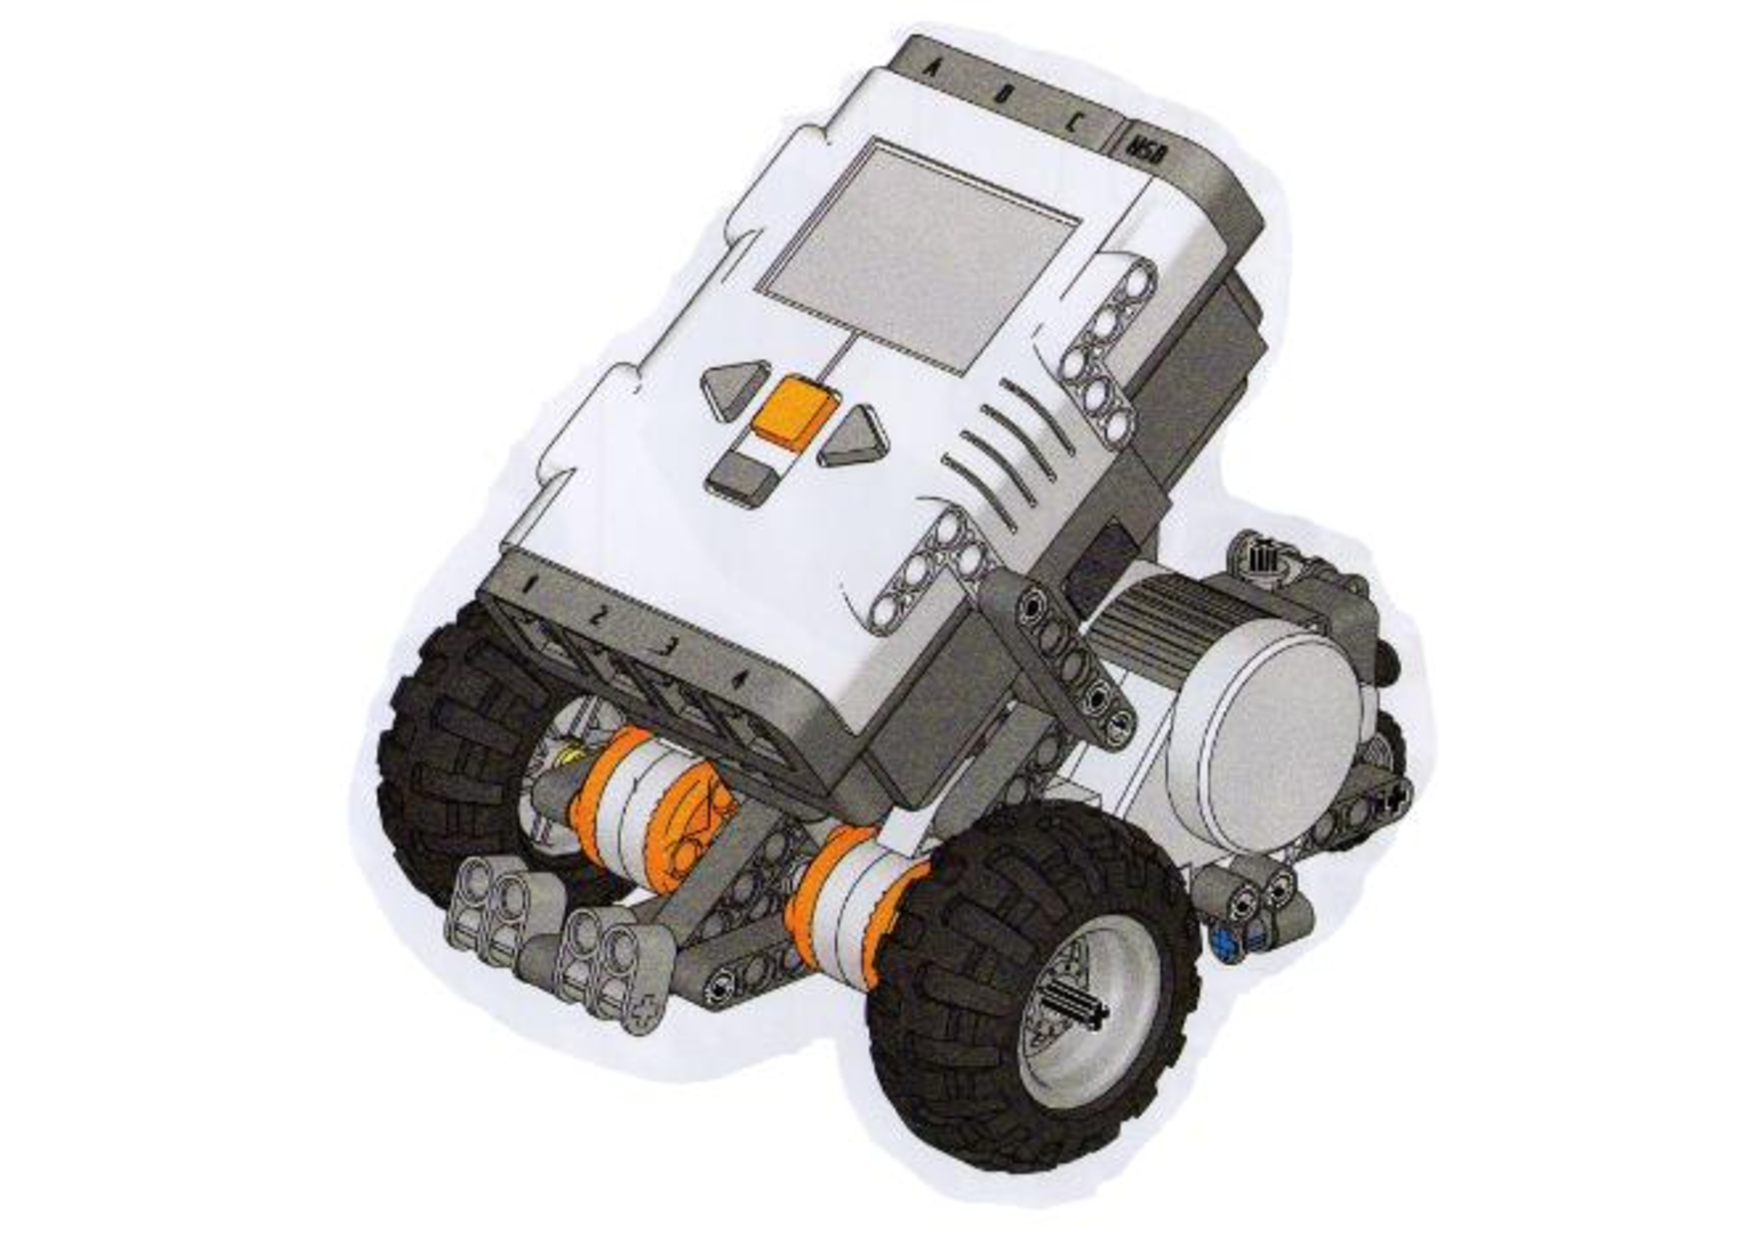
\includegraphics[width=10cm]{./04-figuras/robo}
	\caption{Robô diferencial de duas rodas}
	\label{fig:robo}
\end{figure}

Após feita a modelagem do problema, foram feitas as implementações e os testes, onde seria possível observar se a odometria feita seria suficiente para localizar cada robô do sistema multiagente com precisão e tornar a solução viável. Deve-se levar em consideração que para tanto, foram utilizados os \emph{encoders} óticos acoplados aos motores do \emph{kit Lego Mindstorms\textregistered} os quais possuem uma imprecisão que é da ordem de $\pm$ 1 grau por rotação. 

Concomitantemente, foram realizadas simulações, com o auxílio do software \emph{MATLAB$^{\textregistered}$}, a fim de prever e validar a modelagem feita do problema, desconsiderando os problemas práticos como falha na comunicação e falta de sincronismo entre os robôs, erros dos \emph{encoders} e problemas como saturação do motor e derrapagem das rodas. Outro objetivo dessas simulações é possibilitar que se faça uma comparação entre o sistema real e o seu modelo idealizado.

\section{Modelo Matemático}
\label{sec:modMatematico}
Para introduzir a dinâmica dos robôs móveis utilizados, inicialmente o robô será considerado como um uniciclo, um elemento pontual. O comportamento dinâmico de um robô móvel não-holonômico do tipo uniciclo, desconsiderando-se as forças e os torques causadores do movimento, pode ser descrito pelas equações abaixo:

\begin{equation}
	\dot{x} = v\cos(\theta) 
	\label{eq:posiçãox}
\end{equation}
\begin{equation}
	\dot{y} = v\sin(\theta)
	\label{eq:posiçãoy}
\end{equation}
\begin{equation}
	\dot{\theta} = \omega
	\label{eq:posiçãotheta}
\end{equation}
sendo:
\begin{itemize}
	\item ($x$,$y$) as coordenadas da posição do robô no plano cartesiano;
	\item $\theta$ o ângulo de orientação do robô no plano cartesiano;
	\item $v$ e $\omega$ indicam a velocidade linear e angular do robô, respectivamente, que são as entradas desse sistema dinâmico.	
\end{itemize}

Derivadas dessas equações, surgem as equações (\ref{eq:posiçãoxreal}), (\ref{eq:posiçãoyreal}) e (\ref{eq:posiçãothetareal}) modeladas com base no robô real, que não é um elemento pontual no espaço e sim, um robô diferencial de duas rodas com uma restrição não holonômica. Elas serão utilizadas para gerar as trajetórias dos robôs no ambiente \emph{MATLAB$^{\textregistered}$} e verificar se elas são compatíveis com o caminho percorrido pelos robôs no mundo real. 

As equações que descrevem a posição do robô em função dos giros de cada roda são dadas por:
\begin{subequations}
	\begin{equation}
	x_{k+1} = x_{k} + \dfrac{D_{r} + D_{l}}{2}\cos(\theta_{k}) 
	\label{eq:posiçãoxreal}
	\end{equation}
	\begin{equation}
	y_{k+1} = y_{k} + \dfrac{D_{r} + D_{l}}{2}\sin(\theta_{k}) 
	\label{eq:posiçãoyreal}
	\end{equation}
	\begin{equation}
	\theta_{k+1} = \theta_{k} + \dfrac{D_{r} - D_{l}}{L}
	\label{eq:posiçãothetareal}
	\end{equation}
	\label{eq:posicaorealEnc}
\end{subequations}
sendo, $y_{k+1}$ e $y_{k}$ a coordenada $y$ do robô no instante $k$ e no instante $k+1$; $\theta_{k+1}$ e $\theta_{k}$ o sentido do robô no instante $k$ e no instante $k+1$; $D_{r}$ e $D_{l}$ a distância que a roda direita e esquerda percorreram no instante de tempo entre $k$ e $k+1$, respectivamente; E $L$ o tamanho do eixo das rodas do robô;
%\begin{itemize}
%	\item $y_{k+1}$ e $y_{k}$ a coordenada $y$ do robô no instante $k$ e no instante $k+1$;
%	\item $\theta_{k+1}$ e $\theta_{k}$ o sentido do robô no instante $k$ e no instante $k+1$;	
%	\item $D_{r}$ e $D_{l}$ a distância que a roda direita e esquerda percorreram no instante de tempo entre $k$ e $k+1$, respectivamente;
%	\item $L$ o tamanho do eixo das rodas do robô;
%\end{itemize}

Em que a \autoref{eq:posiçãoxreal} indica que a posição atual do robô em $x$ é igual a posição do robô anterior em $x$ mais a média da distância percorrida por ambas as rodas multiplicado pelo cosseno do ângulo de orientação anterior do robô. Analogamente, a \autoref{eq:posiçãoyreal} descreve a posição em $y$ atual do robô como a posição em $y$ anterior do robô mais a média das distâncias percorridas pelas rodas multiplicada pelo seno do ângulo de orientação do robô no instante anterior. Já a \autoref{eq:posiçãothetareal} indica que o ângulo atual de orientação do robô é igual ao ângulo anterior mais a diferença entre a distância percorrida pelas rodas divido sobre a distância entre as rodas. 

Tendo em vista que a odometria será feita utilizando-se os \emph{encoders} da própria plataforma e o sistema será realimentado com essas medidas, é de extrema importância que a trajetória descrita no mundo real e a registrada pelo robô, utilizando-se os \emph{encoders}, sejam significativamente semelhantes. Caso contrário, a realimentação do sistema estará incorreta, comprometendo seriamente, e por que não dizer inviabilizando, o controle do sistema. 

Dado que a velocidade linear e angular de um robô como o do modelo utilizado neste trabalho é dada pela velocidade angular de cada uma das suas rodas unidirecionais, tem-se nas equações (\ref{eq:vConv}) e (\ref{eq:wConv}) a função que descreve a velocidade linear e angular do robô a partir da velocidade angular de suas rodas. Em que a velocidade linear é dada por
\begin{equation}
	v = \dfrac{(\omega_{r} + \omega_{l}) rp}{2}
	\label{eq:vConv}
\end{equation}
Sendo a média da soma das velocidades de cada roda dadas em $rad/s$, multiplicado pelo raio da roda. E a velocidade angular é dada pela diferença das rodas  direita e esquerda  multiplicada pelo raio da roda e dividido pelo tamanho do eixo, como indicado abaixo:
\begin{equation}
	\omega = \dfrac{(\omega_{r} - \omega_{l}) rp}{L}
	\label{eq:wConv}
\end{equation}
em que:
\begin{itemize}
	\item $v$ é a velocidade linear do robô;
	\item $\omega$ é a velocidade angular do robô;
	\item $\omega_{r}$ é a velocidade angular da roda direita do robô;
	\item $\omega_{l}$ é a velocidade angular da roda esquerda do robô;
	\item $r_{p}$ é o raio da roda do robô;
	\item $L$ é a distância entre as rodas unidirecionais do robô.
\end{itemize}

\section{Problema 1: Varredura de área em paralelo}
\label{sec:P1}
O primeiro problema consiste em: dada uma frota de \emph{N} robôs, esses robôs devem se alinhar horizontalmente e seguir em linha reta, andando paralelamente, utilizando a estrutura já citada na seção \ref{sec:controleFormacao}, denominada \emph{"In Line"}. Primeiro, este problema será modelado considerando a estrutura de comunicação da rede e permitindo apenas velocidades lineares em que o robô pode se deslocar em linha reta e podendo imprimir velocidades negativas e positivas. 

Considerando-se \emph{N} robôs separados por uma distância $\Delta$$y$ no eixo $y$, cada um em um ponto distinto no eixo $x$, como mostrado na \autoref{fig:p1} (a), a tropa deve se alinhar paralelamente e seguir andando paralelamente com uma velocidade $v_{d}$ constante.

\begin{figure}[!htb]
	\centering
	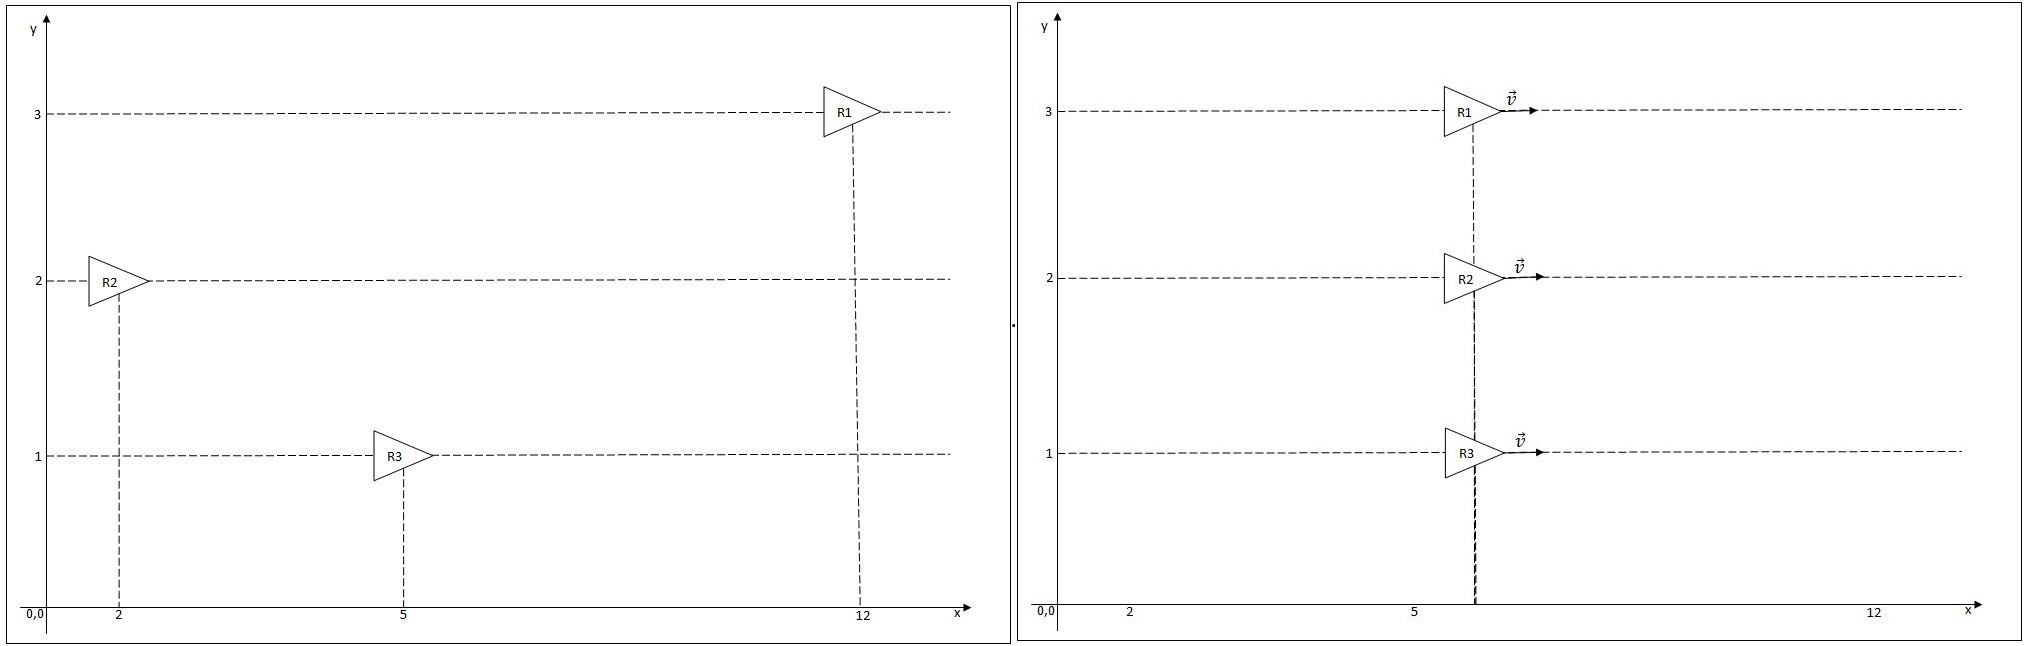
\includegraphics[width=16cm]{./04-figuras/p1}
	\caption{Problema 1: Fig.(a): Sistema no instante $t_{i}$. Fig.(b): Sistema no instante $t_{2}$, em que $t_{2}$$>$$t_{1}$.}
	\label{fig:p1}
\end{figure}

Para alinhar os robôs pode-se usar diferente equações para se definir o erro de posicionamento do robô. Embora não seja a intenção deste trabalho implementar uma rede distribuída, uma forma interessante de se fazer isto é levar em consideração uma rede distribuída, onde um robô não possui a localização de todos os outros robôs e não precisa de uma dependência com um determinado mestre. Desta forma, podemos definir os erros entre os robôs vizinhos conforme a estrutura da rede, como será explicado mais a diante.

Existem diversos tipos de estruturas de rede como mostrado na \autoref{fig:redes}, em que cada círculo indica um robô e as setas indicam a comunicação que ocorre entre eles. Ou seja, na \autoref{fig:redeserial1} o robô 1 troca mensagens somente com o robô 2, que por sua vez, troca mensagens com o robô 1 e 3 e assim sucessivamente. Na \autoref{fig:redenxt} a rede é como a implementada neste trabalho, em que o mestre se comunica com todos os escravos e os escravos não trocam mensagem entre sí. Já na \autoref{fig:rededistr} a rede é descentralizada, o robô 1 troca mensagens com o robô 2 e 3. O robô 3 por sua vez, troca mensagens com o robô 4 e 5. E por fim, na \autoref{fig:redeisolada} há duas redes, sendo que uma não troca mensagem com a outra.
\begin{figure}[!htb]
	\centering
	\begin{subfigure}{.5\textwidth}
		\centering
		\includegraphics[width=.9\linewidth]{./04-figuras/RedeSerial}
		\caption{Rede em Linha Poligonal}
		\label{fig:redeserial1}
	\end{subfigure}%
	\begin{subfigure}{.5\textwidth}
		\centering
		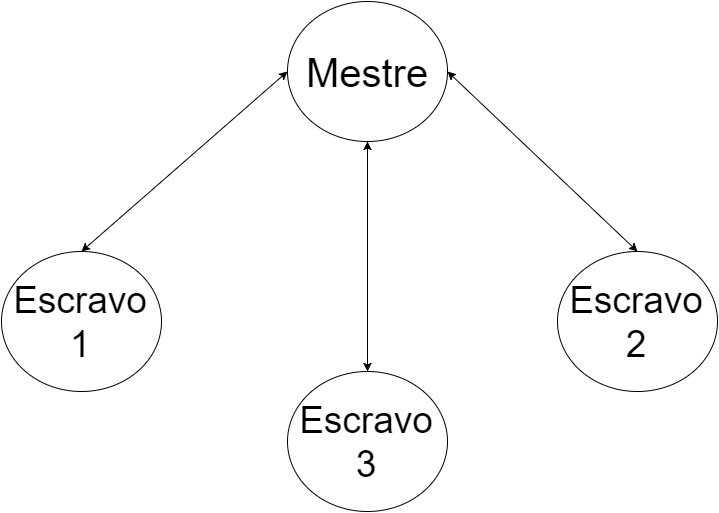
\includegraphics[width=.9\linewidth]{./04-figuras/RedeNXC}
		\caption{Rede Mestre/Escravo}
		\label{fig:redenxt}
	\end{subfigure}
	\begin{subfigure}{.45\textwidth}
		\centering
		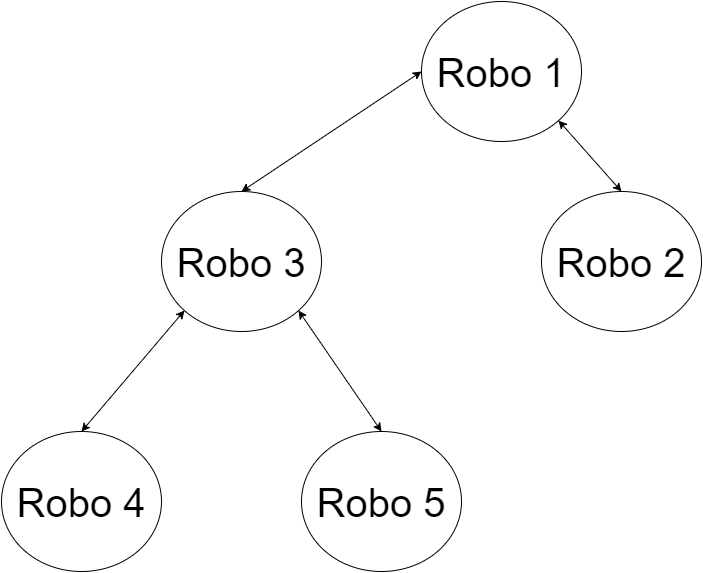
\includegraphics[width=.9\linewidth]{./04-figuras/RedeDistribuida}
		\caption{Rede Descentralizada}
		\label{fig:rededistr}
	\end{subfigure}
	\begin{subfigure}{.45\textwidth}
		\centering
		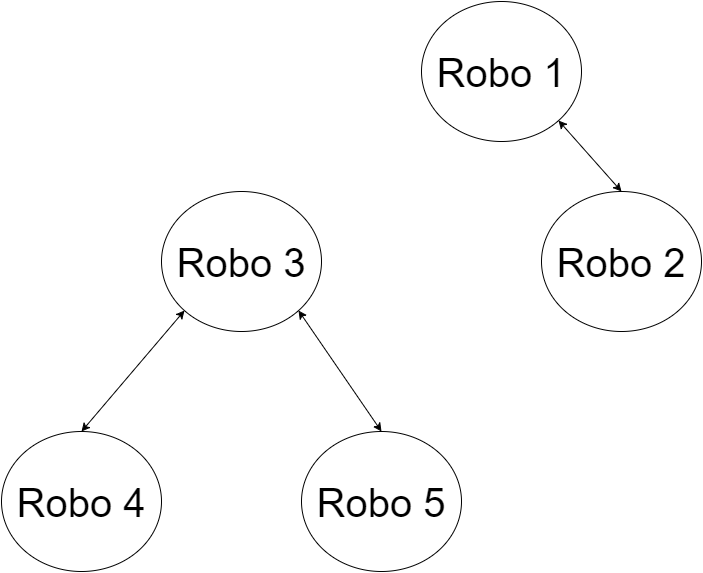
\includegraphics[width=.9\linewidth]{./04-figuras/RedeIsolada}
		\caption{Redes Isoladas}
		\label{fig:redeisolada}
	\end{subfigure}
	\caption{Estruturas de Rede}
	\label{fig:redes}
\end{figure}

Sendo assim, uma forma de se alinhar a tropa seria definir a velocidade de cada $robô_{j}$ de acordo com o erro entre a sua posição e a posição dos robôs vizinhos, aqueles com os quais o $robô_{j}$ troca mensagens.Assim, a velocidade do j-ésimo robô é dada por:
\begin{equation}
	v_{j} = v_{d} + k_{j} \sum\limits_{i = 1}^{n_{j}} e_{i,j}
	\label{eq:velP1}
\end{equation}
em que:
\begin{itemize}
	\item $j$ é o número do robô;
	\item $n_{j}$ é o número de vizinhos do j-ésimo robô;
	%\item $x_{i}$ é a posição do vizinho $i$ daquele robô;
	\item $e_{i,j}$ é a diferença entre a posição no $eixo$ $x$ do j-ésimo robô e seu i-ésimo vizinho.
\end{itemize}

%Supondo uma tropa de três robôs utilizando a rede centralizada utilizada neste trabalho, onde o robô 2 é o mestre e todos os robôs estão orientados no mesmo sentido do eixo x, as velocidades de cada robô devem variar de acordo com o erro de posicionamento do mesmo no eixo x, conforme a distância entre os robôs, como mostrado nas  equações (\ref{eq:vel1P1}), (\ref{eq:vel2P1}) e (\ref{eq:vel3P1}). Essas equações fazem com que o robô mais adiantado da frotase desloque com uma velocidade menor que os outros robôs, tendendo a se aproximar dos mesmos; em contrapartida os robôs que estão "atrasados" se deslocam com uma velocidade maior, até que o erro entre eles seja zero e os mesmos caminhem com velocidade constante. 
Supondo uma tropa de três robôs utilizando a rede centralizada utilizada neste trabalho, onde o robô 2 é o mestre e todos os robôs estão orientados no mesmo sentido do eixo x, as velocidades de cada robô devem variar de acordo com o erro de posicionamento do mesmo no eixo x, conforme a distância entre os robôs, como mostrado nas  equações abaixo:
\begin{equation}
v_{1} = v_{d} + k_{1} e_{2,1}
\label{eq:vel1P1}
\end{equation}
\begin{equation}
v_{2} = v_{d} + k_{2} (e_{1,2} + e_{3,2})
\label{eq:vel2P1}
\end{equation}
\begin{equation}
v_{3} = v_{d} + k_{3} e_{1,3}
\label{eq:vel3P1}
\end{equation}
sendo,
\begin{itemize}
	\item $v_{1}$, $v_{2}$ e $v_{3}$ são as velocidades que cada robô deve possuir para assumir a formação \emph{in line};
	\item $v_{d}$ é a velocidade que a frota deve assumir após estar alinhada;
	\item $k_{1},k_{2},k_{3}$ são as constantes de ganho proporcional do controlador;
	\item E as variáveis de erro são calculadas, obtendo se a diferença entre a posição dos robôs no eixo $x$, como demonstrado na equação abaixo:	
\end{itemize}
\begin{equation}
erro_{i,j} = x_{i} - x_{j}
\label{eq:errp1}
\end{equation}

 Essas equações fazem com que o robô mais adiantado da frotas e desloque com uma velocidade menor que os outros robôs, tendendo a se aproximar dos mesmos; em contrapartida os robôs que estão "atrasados" se deslocam com uma velocidade maior, até que o erro entre eles seja zero e os mesmos caminhem com velocidade constante. 

É importante notar que ao abordar o problemas desta maneira elimina-se a possibilidade de colisão entre os robôs, que estão inicialmente separados no eixo y e alinhados no mesmo sentido, e assim seguem, visto que os mesmos não imprimem velocidade angular. Desta forma, tem-se um problema bem didático para ser abordado inicialmente. %Posteriormente, será mostrado como o  problema pode ser abordado desconsiderando a restrição de estarem separados inicialmente. %sendo abordado de outra forma.

Outra forma de abordar esse problema é pensar que existe uma reta perpendicular ao eixo $x$ (supondo que deseja-se deslocar a frota no mesmo sentido que o eixo das abscissas), tal que essa reta é dada pela equação
\begin{equation}
x_{d} (t) = \dfrac{(max(x_{frota (t)}) + min(x_{frota (t)}))}{2};
\label{eq:xdp1}
\end{equation}
onde:
\begin{itemize}
	\item $x_{frota}$ é um vetor com todas as coordenadas do eixo $x$ dos robôs da frota; 
\end{itemize}
Em que o valor de $x$ desejado ($x_{d}$) é a media das posições entre os robôs mais distantes entre si (considerando-se o posicionamento com relação ao eixo das abscissas). Todos os robôs devem alcançar a posição $(x_{d},y_{j})$, em que o valor de $y_{j}$ é a coordenada vertical do j-ésimo robô,sendo que $y_{p} \neq y_{q}$, se $p \neq q$. Sendo assim, todos os robôs seriam alinhados e a partir dai seguiriam em linha reta, cumprindo o objetivo.

\section{Problema 2: Circulando um alvo}

%O segundo problema consistem em dado um alvo de posiçao $(x,y)$ no plano, a frota deve se locomover até o alvo e o circular, mantendo uma distância $R$ do alvo, com determinada velocidade angular que deve variar de acordo com o tamanho da frota.  
O segundo problema consiste em guiar um time de robôs a localizar e circular, a uma distância \emph{R}, um alvo localizado em uma determinada posição (\emph{x,y}) do plano, como mostrado na \autoref{fig:esq2}. E tem como objetivo secundário ajustar a formação da tropa de robôs que deve se reajustar de acordo com o número de robôs \emph{N}, para que continue cobrindo com eficiência a fronteira. Ou seja, caso um ou mais robôs saiam da rede, a frota irá se reajustar para que cada robô tenha a mesma distância entre si e assim, não fique uma grande parte da fronteira sem cobertura, como demostrado na \autoref{fig:sistema}, que representa uma frota de quatro robôs andando ao redor do alvo, quando então, um dos robôs falha. O sistema, então, se reajusta para adaptar-se à rede de apenas três robôs.

\begin{figure}[!htb]
	\centering
	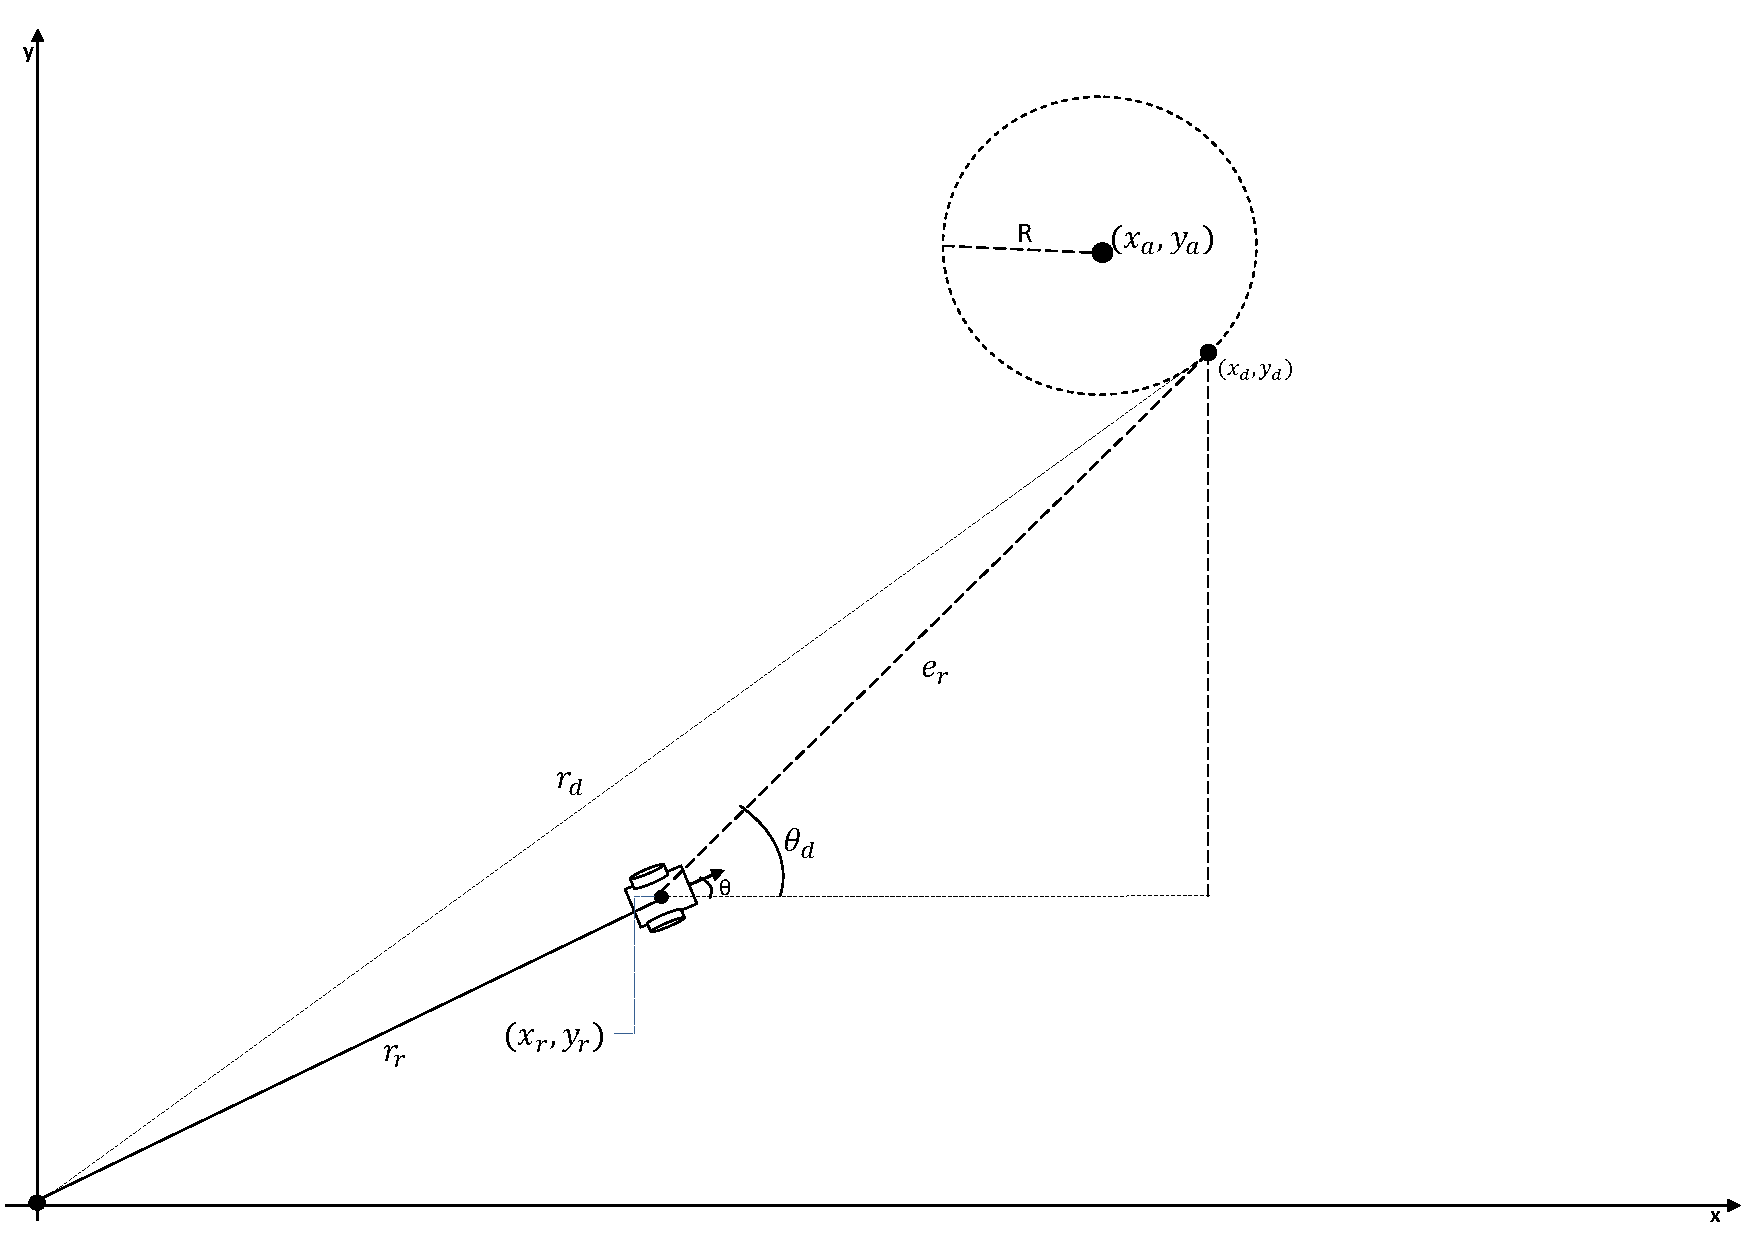
\includegraphics[width=1.0\textwidth]{./04-figuras/esqSistema}
	\caption{Esquema do sistema do ponto de vista de apenas um agente}
	\label{fig:esq2}
\end{figure}

\begin{figure}[!htb]
	\centering
	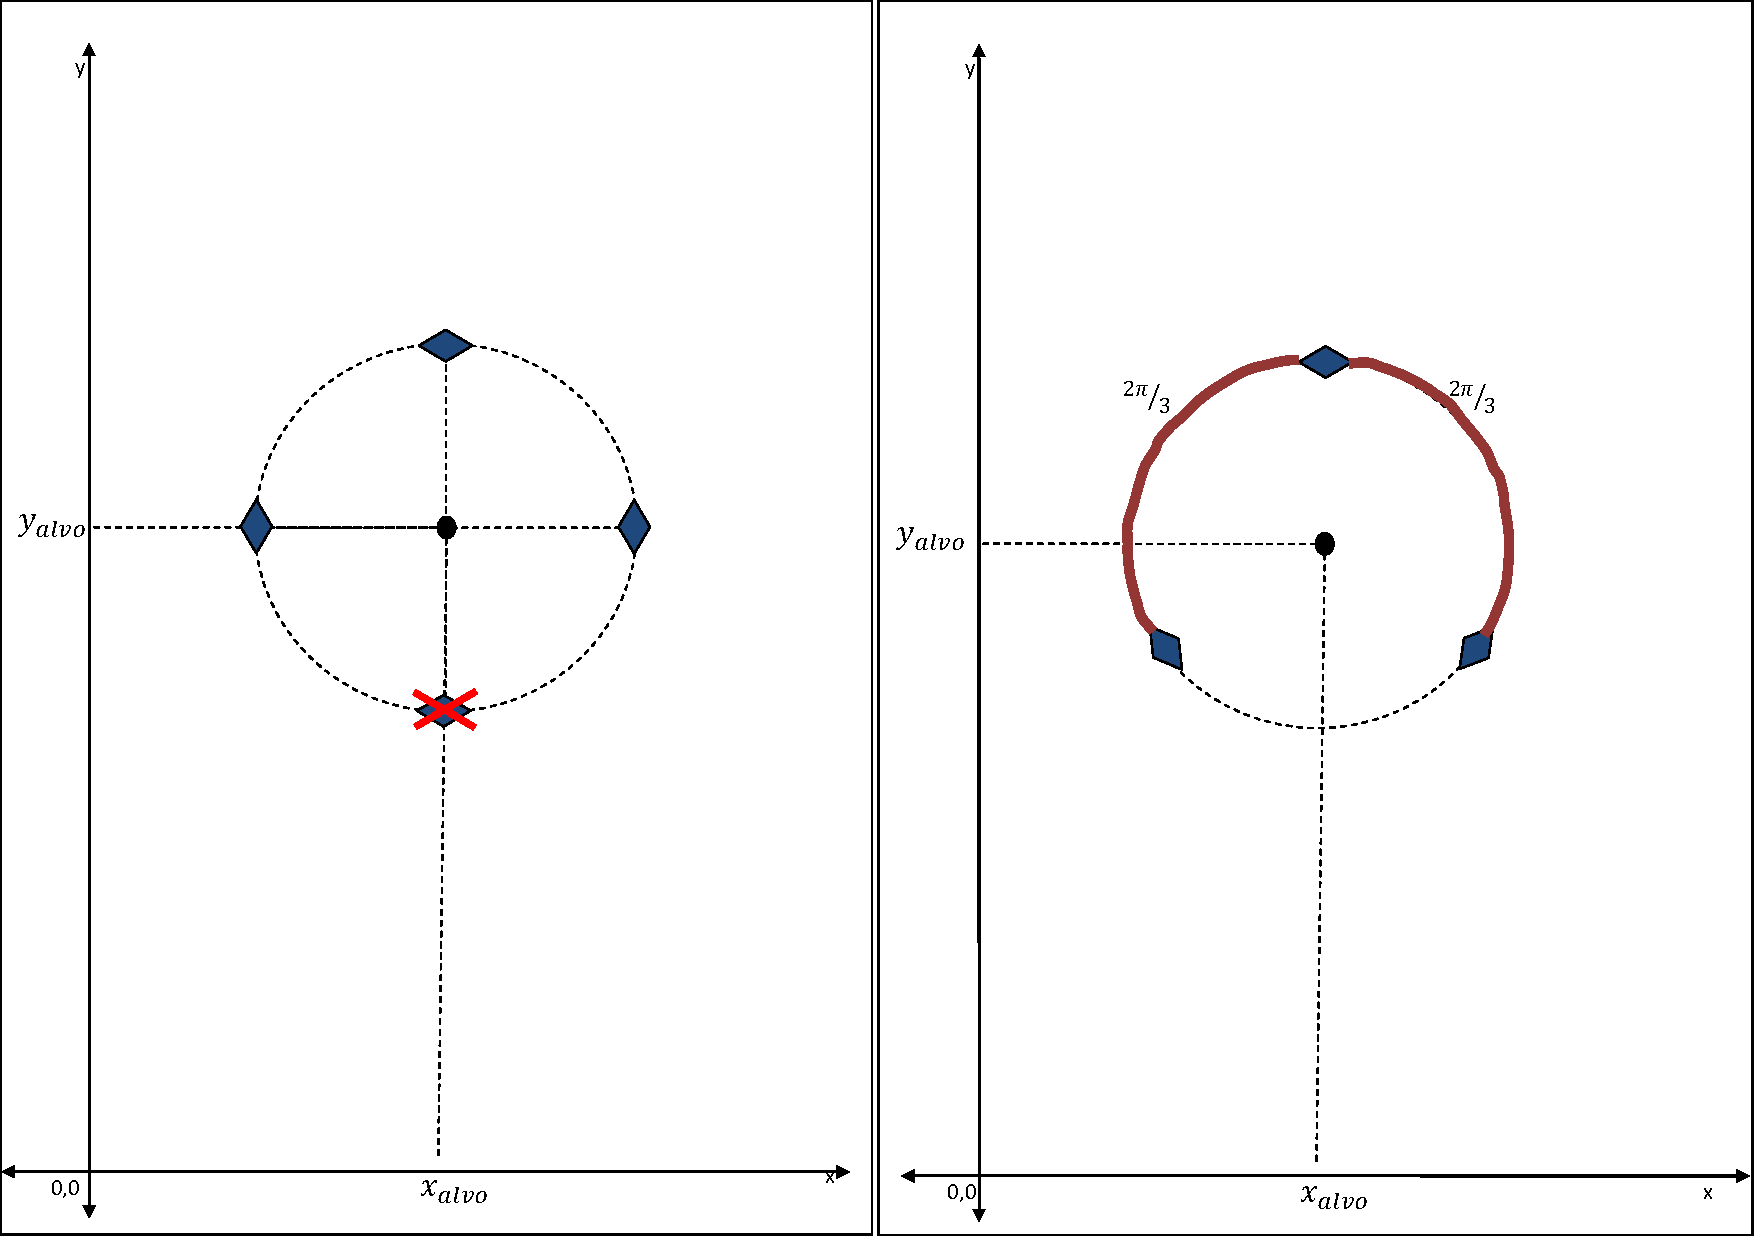
\includegraphics[width=1.0\textwidth]{./04-figuras/sistema}
	\caption{Reconfiguração do sistema mediante falha de um agente}
	\label{fig:sistema}
\end{figure}

Para calcular a posição desejada de cada robô ao redor do alvo, usam-se as equações (\ref{eq:xd_p2}), (\ref{eq:yd_p2}) e (\ref{eq:defj}) que como pode ser visto levam em consideração a posição do alvo ($x_{a},y_{a}$), o raio ($R$) que é a distância com que se deseja circular o alvo, a velocidade angular ($\omega$) com que se deseja percorrer o perímetro (a essa velocidade está associado um período $T$ dado por $2\pi/\omega$) e, além disso, levam em consideração o tamanho da frota e a numeração de cada robô na mesma. O segundo termo adicionado a $\omega t$ significa exatamente a distância angular que cada par de robôs adjacentes terá entre si, que é de $\dfrac{2\pi}{n}$.

\begin{subequations}
\begin{equation}
x_{d} = x_{a} + R\hspace{3pt}cos\left(\omega t + \dfrac{(j-1)2\pi}{n}\right)
\label{eq:xd_p2}
\end{equation}
\begin{equation}
y_{d} = y_{a} + R\hspace{2pt}sin\left(\omega t + \dfrac{(j-1)2\pi}{n}\right)
\label{eq:yd_p2}
\end{equation}
\begin{equation}
j = {1,...,n}
\label{eq:defj}
\end{equation}
\label{eq:posDesejada_p2}
\end{subequations}
sendo:
\begin{itemize}
	\item ($x_{a},y_{a}$) é a posição do alvo;
	\item $R$ é o raio do círculo em torno do alvo;
	\item $\omega$ é a velocidade angular com que deseja-se percorrer o círculo;
	\item $t$ é o tempo decorrido em segundos;
	\item $n$ é o número de robôs da frota;
	\item $j$ é a numeração do robô na frota. 
\end{itemize}

À medida que o sistema se estabiliza, a trajetória do robô tende a convergir para um movimento circular uniforme ao redor do alvo, conforme está ilustrado na \autoref{fig:sistEst}. Ou seja, a velocidade linear ($v$) tende a se igualar à velocidade angular ($\omega$) vezes o raio ($R$) de distância do alvo. 

\begin{figure}[!htb]
	\centering
	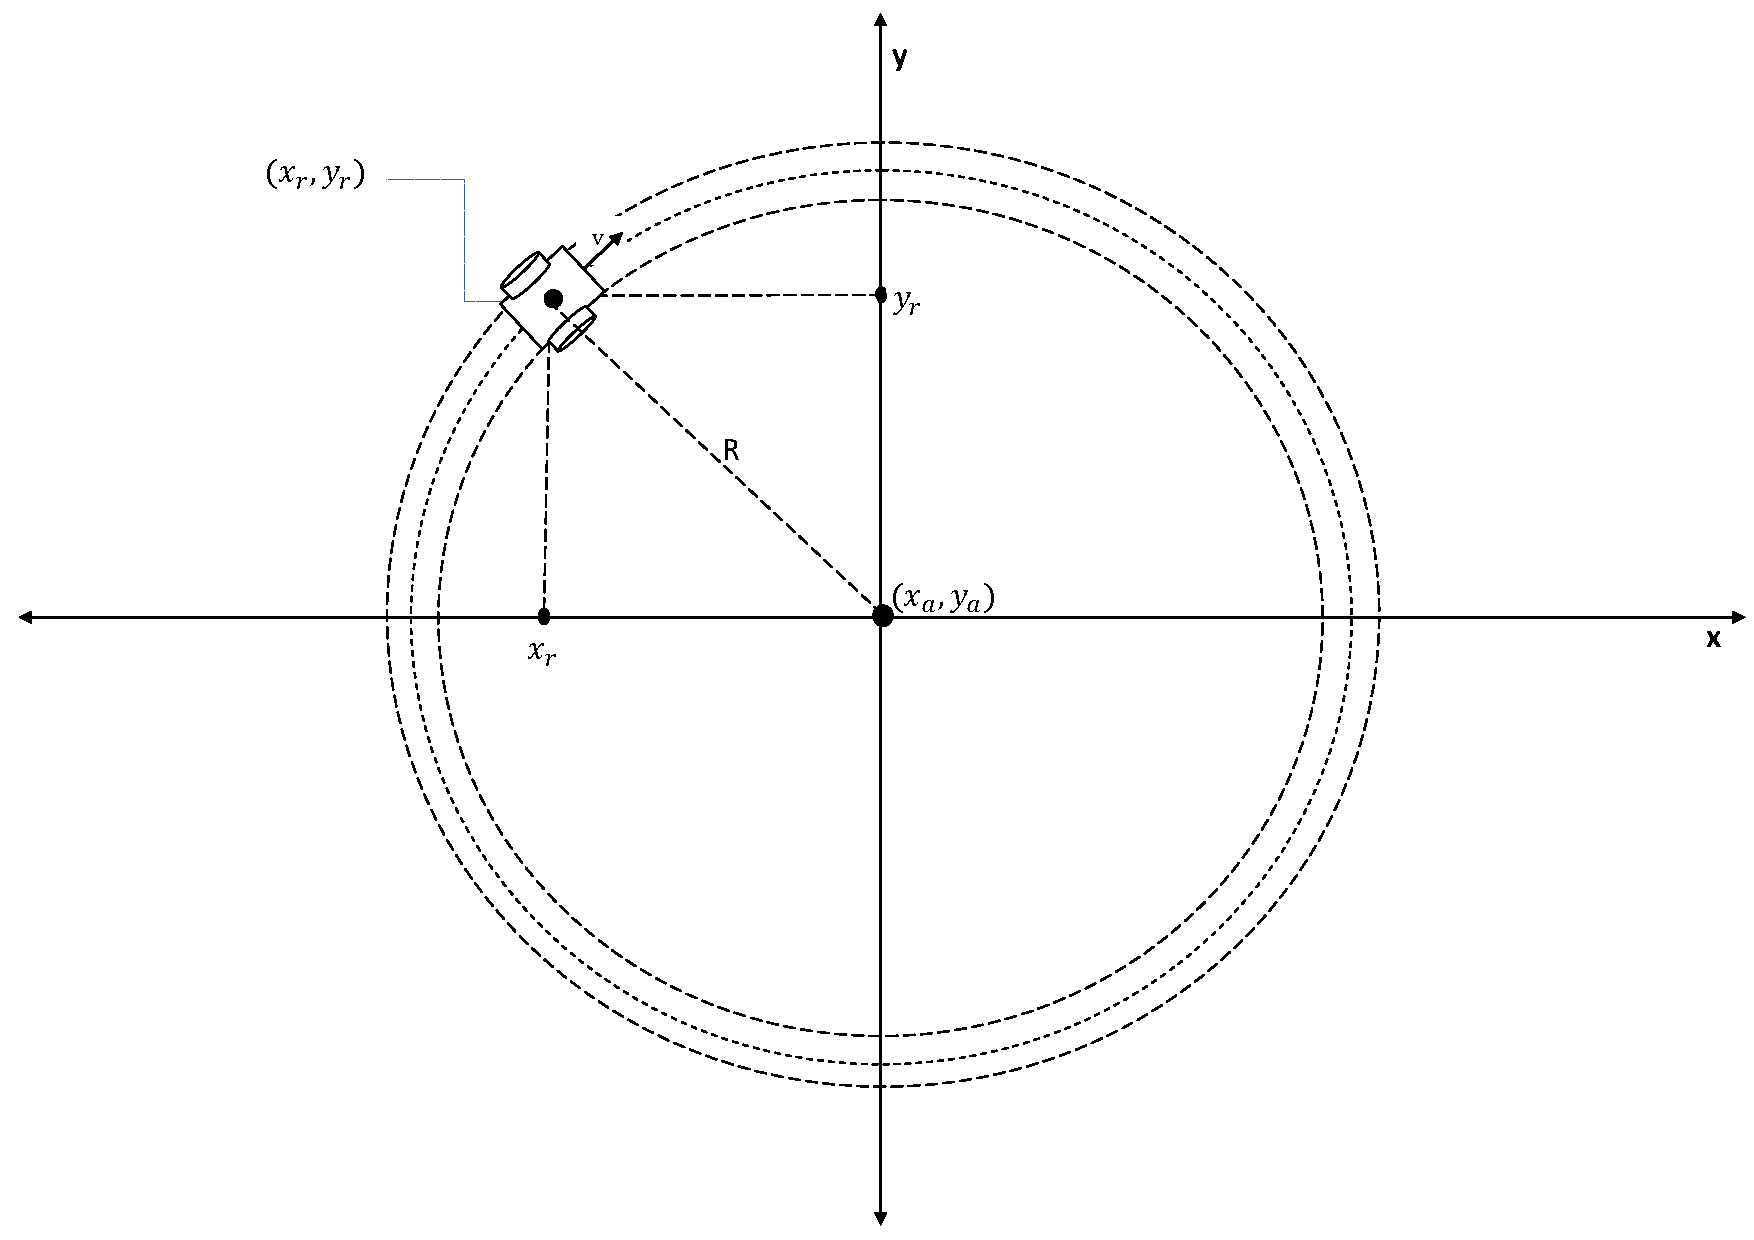
\includegraphics[width=1.0\textwidth]{./04-figuras/sistEstavel2}
	\caption{Representação do sistema estabilizado com um único agente}
	\label{fig:sistEst}
\end{figure}


%\begin{equation}
%\omega = \dfrac{2\pi}{T}
%label{eq:velocangular}
%\end{equation}



